\chapter{Double-Pushout Physics (DPO): The Rule of Rules}
\label{chap:dpo-physics}

There's a moment in every engineer's career when the question stops being \textit{``What is the system?\,''} and becomes \textit{``How does the system change?\,''}

In real work---debugging, compilers, distributed systems, training loops---a static snapshot is rarely the point. You care about what just happened, what happens next, and what breaks when you touch one component.

And sooner or later you hit the uncomfortable fact: most systems don't actually have a definition of \textit{change}. They have a pile of ad-hoc mutations that \textit{usually} behave. Until they don't.

This chapter introduces \textbf{Double-Pushout rewriting (DPO)}: a precise way to describe \emph{legal} structural change. In WARP terms, DPO is the physics of WARP space---the Rule of Rules.\footnote{Earlier drafts referred to WARP graphs as ``recursive metagraphs (RMGs).'' That terminology is retired.}

\section{WARP Graphs Come to Life Through Rules}
\label{sec:warp-life}

WARP graphs give us a rich, nested territory of possible states. But structure alone is inert. A graph without rules is a universe frozen mid-frame: plenty of detail, zero motion.

Computation starts when you add laws.
Rules tell you which local rewrites are allowed, which are forbidden, and what it means to take one step forward.

If the WARP state is the space, DPO is the physics. It turns edges from ``things that exist'' into ``things that \emph{do}.''
And in this book, rules are first-class citizens: they are the operators of the Worldline Algebra.

\section{The Contract of Change: The $L \leftarrow K \rightarrow R$ Span}
\label{sec:warp-contract}

A transformation can't just rewrite structure at random. If a change is going to be meaningful (and not corrupt your universe), it has to respect a contract.

In DPO, that contract is a triplet of graphs called a \emph{span}:
\[
L \leftarrow K \rightarrow R .
\]
Read it like this:

\begin{itemize}
    \item $L$ is what the rule needs to see (the \textbf{pattern}).
    \item $K$ is what the rule promises not to damage (the \textbf{interface}).
    \item $R$ is what the rule installs (the \textbf{result}).
\end{itemize}

\begin{figure}[h]
    \centering
    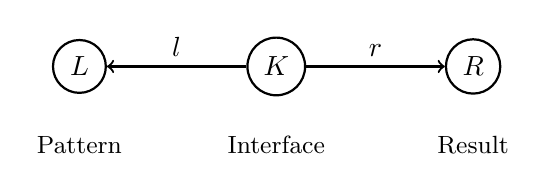
\begin{tikzpicture}[node distance=2.5cm, auto, thick]
        % The Span
        \node (K) [draw, circle] {$K$};
        \node (L) [draw, circle, left of=K] {$L$};
        \node (R) [draw, circle, right of=K] {$R$};

        \draw[->] (K) -- node [above] {$l$} (L);
        \draw[->] (K) -- node [above] {$r$} (R);

        \node [below of=L, node distance=1cm] {\small Pattern};
        \node [below of=K, node distance=1cm] {\small Interface};
        \node [below of=R, node distance=1cm] {\small Result};
    \end{tikzpicture}
    \caption{The DPO span: the fundamental atom of change. The interface $K$ is the seam where the rule must match the surrounding universe.}
    \label{fig:dpo-span}
\end{figure}

$L$ is the precondition. If the current universe can't find a match for $L$, nothing happens. No match, no motion.

$K$ is the heart of the rule. It is the shared boundary that must survive on both sides. Think of $K$ as the seam of a surgical cut: if the seam doesn't line up, the operation is illegal because you can't reattach cleanly.

$R$ is the replacement. The rewrite removes everything in $L$ that isn't part of $K$, then glues in the new structure from $R$ along that same interface.

\section{The Mechanics: Cut a Hole, Then Glue}
\label{sec:dpo-mechanics}

The name \textit{``Double-Pushout''} is not trying to be friendly. It's a category theory term.

The idea, however, is simple:

\begin{enumerate}
    \item Find a match of $L$ inside the current universe $G$.
    \item \textbf{Cut:} remove the part of that match that lies outside the interface $K$, producing an intermediate context $D$.
    \item \textbf{Glue:} attach the replacement $R$ along the same interface, producing the new universe $H$.
\end{enumerate}

People talk about a ``hole'' here for a reason. $D$ is not a metaphorical state. It's the literal remainder of the universe after you've removed the part you're allowed to touch. The interface is still there. The surrounding edges are still there. What's missing is the interior.

If you want a human picture, it's graph surgery: snip out the old piece, keep the boundary, glue in the new piece.

To make this less abstract, here's a toy rule we'll use as a running example. It preserves the boundary nodes $p$ and $q$ (the interface $K$) and swaps the interior $x$ for a new interior $y$:

\begin{figure}[h]
\centering
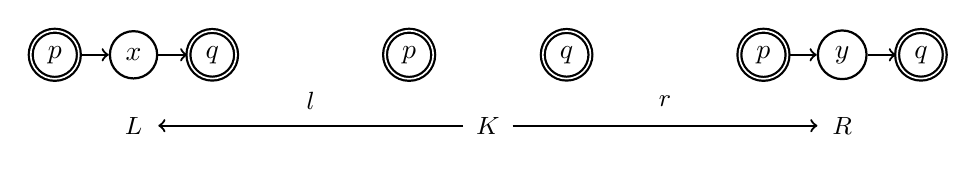
\begin{tikzpicture}[auto, thick, every node/.style={circle,draw,minimum size=6mm}]
    % --- L ---
    \node[double] (Lp) at (0,0) {$p$};
    \node (Lx) at (1.0,0) {$x$};
    \node[double] (Lq) at (2.0,0) {$q$};
    \draw[->] (Lp) -- (Lx);
    \draw[->] (Lx) -- (Lq);
    \node[draw=none, rectangle, font=\small] (Llab) at (1.0,-0.9) {$L$};

    % --- K ---
    \node[double] (Kp) at (4.5,0) {$p$};
    \node[double] (Kq) at (6.5,0) {$q$};
    \node[draw=none, rectangle, font=\small] (Klab) at (5.5,-0.9) {$K$};

    % --- R ---
    \node[double] (Rp) at (9.0,0) {$p$};
    \node (Ry) at (10.0,0) {$y$};
    \node[double] (Rq) at (11.0,0) {$q$};
    \draw[->] (Rp) -- (Ry);
    \draw[->] (Ry) -- (Rq);
    \node[draw=none, rectangle, font=\small] (Rlab) at (10.0,-0.9) {$R$};

    % --- arrows (the span) ---
    \draw[->, thick] (Klab) -- node[above, draw=none, rectangle, font=\small] {$l$} (Llab);
    \draw[->, thick] (Klab) -- node[above, draw=none, rectangle, font=\small] {$r$} (Rlab);
\end{tikzpicture}
\caption{A concrete DPO rule. The interface $K$ (double-bordered nodes) must survive the rewrite. Everything in $L$ outside of $K$ is removed; everything in $R$ outside of $K$ is added.}
\label{fig:dpo-rule-example}
\end{figure}


\begin{figure}[h]
\centering
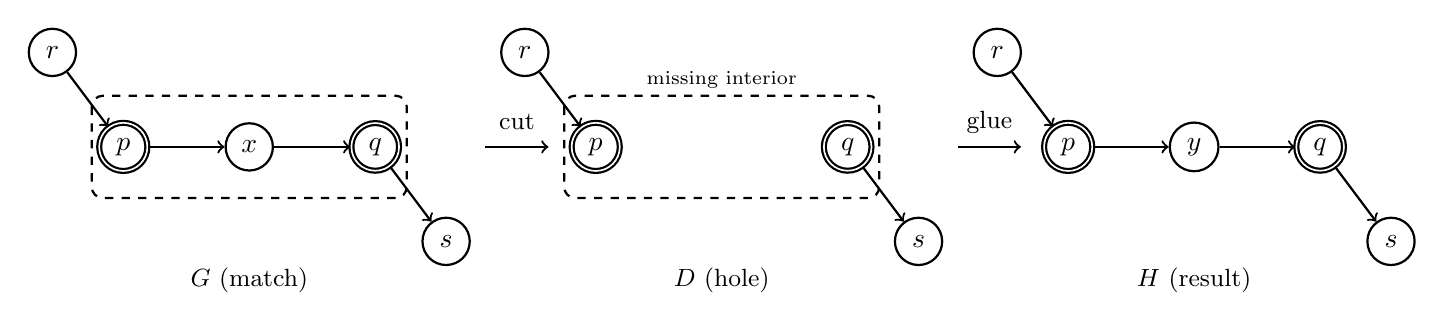
\begin{tikzpicture}[auto, thick, every node/.style={circle,draw,minimum size=6mm}]
    % --- G ---
    \begin{scope}
        \node[double] (Gp) at (0,0) {$p$};
        \node (Gx) at (1.6,0) {$x$};
        \node[double] (Gq) at (3.2,0) {$q$};
        \node (Gr) at (-0.9,1.2) {$r$};
        \node (Gs) at (4.1,-1.2) {$s$};
        \draw[->] (Gr) -- (Gp);
        \draw[->] (Gp) -- (Gx);
        \draw[->] (Gx) -- (Gq);
        \draw[->] (Gq) -- (Gs);
        \draw[dashed, rounded corners] (-0.4,0.65) rectangle (3.6,-0.65);
        \node[draw=none, rectangle, font=\small] at (1.6,-1.7) {$G$ (match)};
    \end{scope}

    % arrow (cut)
    \draw[->, thick] (4.6,0) -- node[above, draw=none, rectangle, font=\small] {cut} (5.4,0);

    % --- D ---
    \begin{scope}[xshift=6cm]
        \node[double] (Dp) at (0,0) {$p$};
        \node[double] (Dq) at (3.2,0) {$q$};
        \node (Dr) at (-0.9,1.2) {$r$};
        \node (Ds) at (4.1,-1.2) {$s$};
        \draw[->] (Dr) -- (Dp);
        \draw[->] (Dq) -- (Ds);
        \node[draw=none, rectangle, font=\small] at (1.6,-1.7) {$D$ (hole)};

        % visual hint of the missing interior
        \draw[dashed, rounded corners] (-0.4,0.65) rectangle (3.6,-0.65);
        \node[draw=none, rectangle, font=\scriptsize] at (1.6,0.85) {missing interior};
    \end{scope}

    % arrow (glue)
    \draw[->, thick] (10.6,0) -- node[above, draw=none, rectangle, font=\small] {glue} (11.4,0);

    % --- H ---
    \begin{scope}[xshift=12cm]
        \node[double] (Hp) at (0,0) {$p$};
        \node (Hy) at (1.6,0) {$y$};
        \node[double] (Hq) at (3.2,0) {$q$};
        \node (Hr) at (-0.9,1.2) {$r$};
        \node (Hs) at (4.1,-1.2) {$s$};
        \draw[->] (Hr) -- (Hp);
        \draw[->] (Hp) -- (Hy);
        \draw[->] (Hy) -- (Hq);
        \draw[->] (Hq) -- (Hs);
        \node[draw=none, rectangle, font=\small] at (1.6,-1.7) {$H$ (result)};
    \end{scope}
\end{tikzpicture}
\caption{A cut-and-glue view of one DPO step. The dashed box marks the matched region. The double-bordered nodes are the interface: they stay. The cut removes the interior. The glue installs a replacement interior along the same boundary.}
\label{fig:dpo-cut-glue}
\end{figure}

If you like the formal square, here it is. You don't have to love it; you only have to know what it guarantees:

\begin{figure}[h]
    \centering
    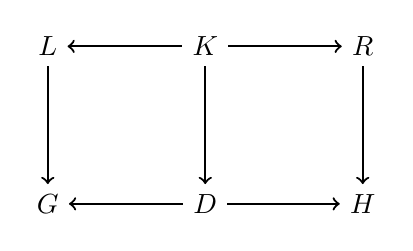
\begin{tikzpicture}[node distance=2cm, auto, thick]
        % Top Row
        \node (L) {$L$};
        \node (K) [right of=L] {$K$};
        \node (R) [right of=K] {$R$};

        % Bottom Row
        \node (G) [below of=L] {$G$};
        \node (D) [below of=K] {$D$};
        \node (H) [below of=R] {$H$};

        % Arrows
        \draw[<-] (L) -- (K);
        \draw[->] (K) -- (R);
        \draw[<-] (G) -- (D);
        \draw[->] (D) -- (H);
        \draw[->] (L) -- (G);
        \draw[->] (K) -- (D);
        \draw[->] (R) -- (H);

        % Square symbols
        \node at (0.5,-1) {$\ulcorner$};
        \node at (2.5,-1) {$\ulcorner$};
    \end{tikzpicture}
    \caption{The Double-Pushout diagram. The rewrite flows from $G$ to $H$ through the intermediate context $D$. The two marked squares are the ``make the hole'' step, and the ``fill the hole'' step.}
    \label{fig:dpo-diagram}
\end{figure}

\section{Safety and the Dangling Condition}
\label{sec:dangling-condition}

In formal DPO theory, a rewrite is only legal if it satisfies the \textbf{dangling condition}. This sounds academic. It is not. It's the exact rule that prevents you from leaving broken pointers in the universe.

The intuition is brutal and familiar: you are not allowed to delete a node while keeping edges that still reference it.

Imagine deleting a server from a network graph. If you don't account for the active connections leading to it, you've just created a nonsense state. DPO enforces this by construction: you may only delete what you have explicitly matched in $L$. If some edge from the outside world still attaches to the part you're trying to remove, then the ``clean cut'' does not exist and the rewrite is blocked.

So DPO fails closed. It refuses to make a move rather than producing a corrupt WARP state.

\begin{figure}[h]
    \centering
    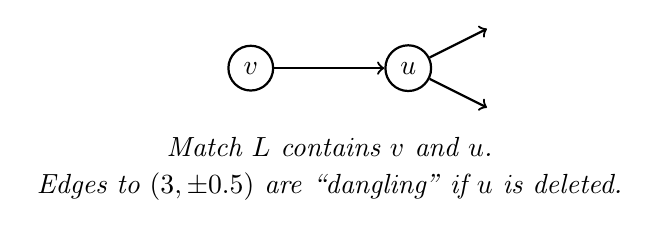
\begin{tikzpicture}[auto, thick, node distance=1.5cm]
        \node[circle, draw] (A) at (0,0) {$v$};
        \node[circle, draw] (B) at (2,0) {$u$};
        \draw[->] (A) -- (B);
        \draw[->] (B) -- (3,0.5);
        \draw[->] (B) -- (3,-0.5);
        \node at (1,-1) {\textit{Match $L$ contains $v$ and $u$.}};
        \node at (1,-1.5) {\textit{Edges to $(3, \pm 0.5)$ are ``dangling'' if $u$ is deleted.}};
    \end{tikzpicture}
    \caption{A visualization of the dangling condition. If the rule attempts to delete $u$, it must also account for all incident edges, or the rewrite is rejected.}
    \label{fig:dangling-visual}
\end{figure}

\section{Interference: Local Laws, Parallel Steps}
\label{sec:interference}

Once you have a notion of legal change, the next question is unavoidable:

\textit{What happens when more than one rule could apply?}

This is where DPO starts to feel less like a rewrite trick and more like physics.
A rule doesn't act on the whole universe. It acts on a \emph{region}---the part of $G$ that matches $L$. That region is the rule's footprint.

Two rewrites \textbf{interfere} when their footprints overlap.
They are trying to touch the same structure, so you're forced to care about order.

But if their matches are disjoint---if they don't overlap---then order stops mattering. Apply rule A then rule B, or rule B then rule A: you get the same result.

Visually, disjoint rewrites form a commuting diamond:

\begin{figure}[h]
    \centering
    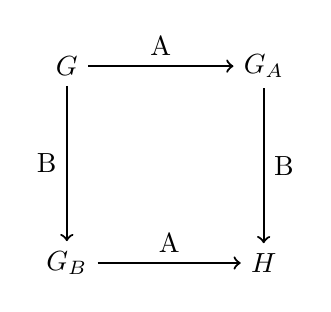
\begin{tikzpicture}[node distance=2.5cm, auto, thick]
        \node (G) {$G$};
        \node (GA) [right of=G] {$G_A$};
        \node (GB) [below of=G] {$G_B$};
        \node (H) [right of=GB] {$H$};

        \draw[->] (G) -- node[above] {A} (GA);
        \draw[->] (G) -- node[left] {B} (GB);
        \draw[->] (GB) -- node[above] {A} (H);
        \draw[->] (GA) -- node[right] {B} (H);
    \end{tikzpicture}
    \caption{When two rules act on disjoint regions, their steps commute: either order lands in the same universe $H$. This is DPO's ``parallelism without races.''}
    \label{fig:dpo-commutation}
\end{figure}


That's not a scheduling hack. It's a property of the laws.
It's also the core reason DPO has a natural \textbf{deterministic concurrent semantics}: parallelism without races, as long as the rules don't collide.

When they \textit{do} collide, you don't get chaos. You get causality.
The graph remembers which change happened first. Later, when we talk about worldlines and rulial paths, this is exactly the kind of structure we're tracking.

\section{Compositionality: Building Worldlines (and Zooming In)}
\label{sec:compositionality}

The true power of DPO is not that it can do one rewrite. It's that it can do many, and do them \emph{modularly}.

Because the interface $K$ makes the boundary explicit, small rules compose into larger pipelines.
You can write a rule for one compiler optimization pass, then compose it with others to evolve the whole program in verifiable steps.
You can build libraries of rules the way we build libraries of functions---except the effects are structural, explicit, and checked.

Now add WARP's recursion and things get weirder (in the good way).
Nodes and edges can contain WARP graphs.
So a ``thing'' that looks atomic from the outside can be an entire universe from the inside.

A rule can target one of these containers in two different ways:

\begin{itemize}
    \item Treat it as an atom and rewrite around it.
    \item Open it and rewrite its interior graph.
\end{itemize}

Do this repeatedly and you get a real zoom effect: evolution not just through time, but through \emph{scale}.
And yes---this is the point where it becomes natural to talk about different effective ``laws'' at different levels of the hierarchy. The rewrite physics can literally change as you move down the stack.

\begin{tcolorbox}[colback=white, colframe=black, title=FOR THE NERDS™]
If your brain is trying to map this to function calls, stop.

A function $f(x)$ is a black box that maps an input value to an output value.
A DPO step is a \emph{structured} edit: match a subgraph, cut it out cleanly, and glue in a replacement along an explicit interface.

The key difference is that DPO preserves the ``rest of the universe'' ($D$) explicitly. That makes interference detectable.
If two matches are disjoint, the rewrites commute. This is where the ``deterministic concurrent semantics'' comes from.
\end{tcolorbox}

\section{Conclusion: The Bridge to Geometry}
\label{sec:bridge-geometry}

WARP gives us structure. DPO gives us motion.
Together, they let us define computational universes and the legal transitions between them.

But the moment you can move, you start asking geometric questions.
Which rewrites are ``close'' to one another?
Which universes are ``neighbors'' in the space of possible evolution?
Which paths are short, and which are needlessly expensive?

DPO already gives us a first lever for this: \textbf{not every change is the same size}.
Some steps tweak a single local feature. Others tear out half a module and replace it.

One crude but useful notion of \textbf{rule weight} is:
\[
w(\rho) = |L \setminus K| + |R \setminus K| ,
\]
the amount of structure you cut out plus the amount you glue in.\footnote{There are richer choices: edge-weighting, typed costs, domain-specific weights. But counting gets us to a metric-shaped intuition fast.}

Once you have weights, you can start talking about paths with cost.
And once you have paths with cost, you're halfway to distance.

That's the bridge to the next chapter.

\textbf{$\rightarrow$ Chapter 5 --- Rulial Space and Rulial Distance}

\textit{Where we give computation a geometry---not literal Euclidean geometry, but a manifold-like space for reasoning about possibility, adjacency, and the limits of what can be computed.}
